\documentclass[boxes]{homework}

% This is a slightly-more-than-minimal document that uses the homework class.
% See the README at http://git.io/vZWL0 for complete documentation.

\name{傅申 PB20000051}        % Replace (Your Name) with your name.
\term{2022 秋}     % Replace (Current Term) with the current term.
\course{算法基础}    % Replace (Course Name) with the course name.
\hwnum{10}          % Replace (Number) with the number of the homework.
\hwname{作业}
\problemname{}
\solutionname{解:}

% Load any other packages you need here.
\usepackage[
    a4paper,
    top = 2.54cm,
    bottom = 2.54cm,
    left = 1.91cm,
    right = 1.91cm,
    includeheadfoot
]{geometry}
\fancyfootoffset{0pt} % make fancyhdr work properly
\usepackage{ctex}
\usepackage{subfigure}
\usepackage{tikz}
\tikzset{
    red/.style={circle, draw=red, fill=red!20, minimum size=1.5em, inner sep=.1em},
    black/.style={circle, draw=black, fill=black!20, minimum size=1.5em, inner sep=.1em},
    level/.style={sibling distance=8em/#1, level distance=2em},
}

\begin{document}
%%%% Problem 13.4-3 %%%%
\problemchap{13}
\problempart{4}
\problemnumber{3}
\begin{problem}
在练习 13.3--2 中, 将关键字 41, 38, 31, 12, 19, 8 连续插入一棵初始的空树中, 从而
得到一棵红黑树. 请给出从该树中连续删除关键字 8, 12, 19, 31, 38, 41 后的红黑树.
\end{problem}
\begin{solution}
    忽略 {\sc Nil} 叶结点, 删除关键字后的红黑树依次如下
    \begin{figure}[htbp]
        \centering
        \subfigure[初始红黑树]{
            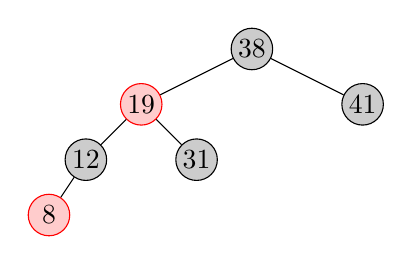
\begin{tikzpicture}
                \node[black] {38}
                child { node[red] {19}
                        child { node[black] {12}
                                child { node[red] {8} }
                                child { node {} edge from parent[draw=none] }
                            }
                        child { node[black] {31} }
                    }
                child { node[black] {41} }
                ;
            \end{tikzpicture}
        }
        \subfigure[删除 8]{
            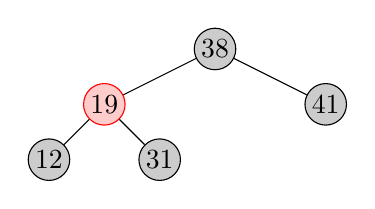
\begin{tikzpicture}
                \node[black] {38}
                child { node[red] {19}
                        child { node[black] {12} }
                        child { node[black] {31} }
                    }
                child { node[black] {41} }
                ;
            \end{tikzpicture}
        }
        \subfigure[删除 12]{
            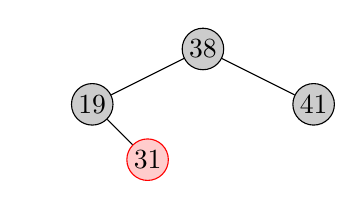
\begin{tikzpicture}
                \node[black] {38}
                child { node[black] {19}
                        child { node {} edge from parent[draw=none] }
                        child { node[red] {31} }
                    }
                child { node[black] {41} }
                ;
            \end{tikzpicture}
        }
        \subfigure[删除 19]{
            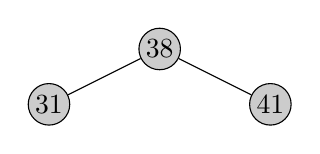
\begin{tikzpicture}
                \node[black] {38}
                child { node[black] {31} }
                child { node[black] {41} }
                ;
            \end{tikzpicture}
        }
        \subfigure[删除 31]{
            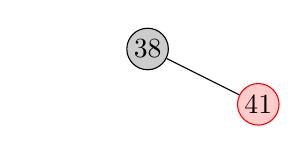
\begin{tikzpicture}
                \node[black] {38}
                child { node {} edge from parent[draw=none] }
                child { node[red] {41} }
                ;
            \end{tikzpicture}
        }
        \subfigure[删除 38]{
            \hspace{.1\textwidth}
            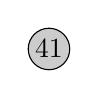
\begin{tikzpicture}
                \node[black] {41}
                ;
            \end{tikzpicture}
            \hspace{.1\textwidth}
        }
        \subfigure[删除 41]{
            \hspace{.1\textwidth}
        }
        \caption{依次删除关键字后的红黑树}
        \label{fig:13.4-3}
    \end{figure}
\end{solution}

%%%% Problem 13.4-7 %%%%
\problempart{4}
\problemnumber{7}
\begin{problem}
假设用 {\sc RB-Insert} 将一个结点 $x$ 插入一棵红黑树, 紧接着又用 {\sc RB-Delete}
将它从树中删除. 结果的红黑树与初始的红黑树是否一样? 证明你的答案.
\end{problem}
\begin{solution}
    不一样, 考虑如下的红黑树.
    \begin{center}
        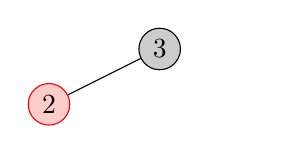
\begin{tikzpicture}
            \node[black] {3}
            child { node[red] {2} }
            child { node {} edge from parent[draw=none] }
            ;
        \end{tikzpicture}
    \end{center}
    插入关键字为 1 的结点后为
    \begin{center}
        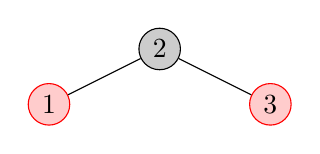
\begin{tikzpicture}
            \node[black] {2}
            child { node[red] {1} }
            child { node[red] {3} }
            ;
        \end{tikzpicture}
    \end{center}
    而再删除 1 后得到
    \begin{center}
        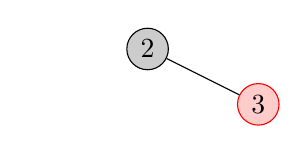
\begin{tikzpicture}
            \node[black] {2}
            child { node {} edge from parent[draw=none] }
            child { node[red] {3} }
            ;
        \end{tikzpicture}
    \end{center}
\end{solution}

%%%% Problem 14.1-2 %%%%
\problemchap{14}
\problempart{1}
\problemnumber{2}
\begin{problem}
对于图 14--1 中的红黑树 $T$ 和关键字 $x.key$ 为 35 的结点 $x$, 说明执行
{\sc OS-Rank}\,($T$, $x$) 的过程.
\end{problem}
\begin{solution}
    首先 $r$ 被初始化为 0, $y$ 初始化为 $x$. 然后进入循环, 第一轮 $y=y.p.left$,
    $r$ 不改变, $y$ 更新为关键字 38 的结点; 第二轮 $y = y.p.right$, $r$ 增加 2,
    $y$ 更新为关键字 30 的结点; 第三轮 $y = y.p.left$, $r$ 不改变, $y$ 更新为关
    键字 41 的结点; 第四轮 $y = y.p.right$, $r$ 增加 13, $y$ 更新为根结点, 循环
    结束. 最后 $r = 15$.
\end{solution}

%%%% Problem 14.1-4 %%%%
\problemnumber{4}
\begin{problem}
写出一个递归过程 {\sc OS-Key-Rank}\,($T$, $k$), 以一棵顺序统计树 $T$ 和一个关键
字 $k$ 作为输入, 要求返回 $k$ 在由 $T$ 表示的动态集合中的秩. 假设 $T$ 的所有关键
字都不相同.
\end{problem}
\begin{solution}
    如下
    \begin{algo}
        \caption{OS-KEY-RANK\,($T$, $k$)}
        $x = T.root$\;
        \uIf{$k = x.key$}{
            \Return{$x.left.size + 1$}\;
        }
        \uElseIf{$k > x.key$}{
            \Return{$x.left.size + 1 + \operatorname{OS-KEY-RANK}(x.right, k)$}\;
        }
        \Else{
            \Return{$\operatorname{OS-KEY-RANK}(x.left, k)$}\;
        }
    \end{algo}
\end{solution}

%%%% Problem 14.2-2 %%%%
\problempart{2}
\problemnumber{2}
\begin{problem}
能否在不影响红黑树任何操作的渐进性能的前提下, 将结点的黑高作为树中结点的一个属性
来维护? 说明如何做, 如果不能, 请说明理由. 如何维护结点的深度?
\end{problem}
\begin{solution}
    因为结点的黑高只与其子结点的黑高和子结点的颜色有关, 所以可以完成题中操作. 在
    插入时, 插入的结点的子结点都是哨兵, 因此其黑高为 1, 并由此向上修改其他结点的
    黑高, 最后在 {\sc Fixup} 过程中对部分结点进行调整. 同理, 在删除时先将结点删
    除, 局部修改黑高并向上传播, 然后在 {\sc Fixup} 过程中对部分结点进行调整.

    而由于结点的深度取决于其父结点的深度, 因此无法维护结点深度.
\end{solution}

%%%% Problem 14.3-4 %%%%
\problempart{3}
\problemnumber{4}
\begin{problem}
给定一棵区间树 $T$ 和一个区间 $i$, 请描述如何在 $O(\min(n, k\lg n))$ 时间内列出
$T$ 中所有与 $i$ 重叠的区间, 其中 $k$ 是输出的区间数. (\textit{提示}: 一种简单的
方法是做若干次查询, 并且在这些查询操作中修改树, 另一种略微复杂点的方法是不对树进
行修改)
\end{problem}
\begin{solution}
    如下, 其中每个结点最多遍历一次, 所以时间是 $O(n)$ 的; 而每次输出一个区间对应
    的递归深度最多为 $\lg n$, 因此时间是 $O(k\lg n)$ 的.
    \begin{algo}
        \caption{INTERVALS-SEARCH\,($T$, $i$)}
        $x = T.root$\;
        \If{$i$ overlaps $x.int$}{
            Print $x.int$\;
        }
        \If{$x.left \neq T.nil$ \textbf{and} $x.left.max \geqslant i.low$}{
            $\operatorname{INTERVALS-SEARCH} (x.left, i)$\;
        }
        \If{$x.right \neq T.nil$ \textbf{and} $x.int.low \leqslant i.high$
            \textbf{and} $x.right.max \geqslant i.low$}{
            $\operatorname{INTERVALS-SEARCH} (x.right, i)$\;
        }
    \end{algo}
\end{solution}

\end{document}
